
\subsection{Arsitektur Perangkat Lunak}
	\label{final-arch-tech}
	Sifat rancang bangun aplikasi ini yang bersifat \textit{incremental} terhadap hasil analisa ilmiah dan pengalaman penulis sendiri. Sifat \textit{incremental} tersebut berdampak perubahan arsitektur dan pemilihan teknologi yang digunakan selama masa pengerjaan aplikasi. Subbab ini akan merangkum subbab \ref{tech-analysis} dan subbab \ref{tech-options} dalam bentuk sebuah diagram visualisasi. Rangkuman tersebut berupa visualisasi arsitektur digabungkan dengan teknologi yang digunakan. Selain itu, penulis juga menambahkan visualisasi warna untuk mempermudah pemahaman pembaca.
	
	\begin{figure}[H]
		\centering
		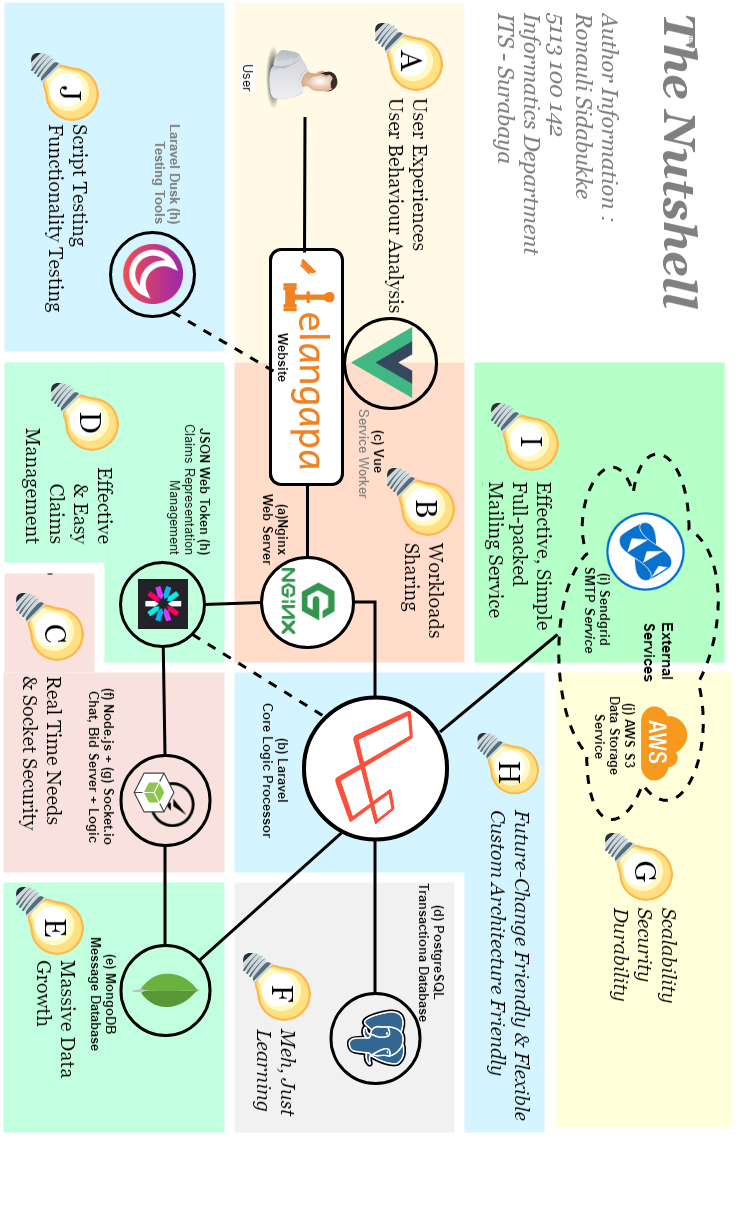
\includegraphics[width=.8\textwidth]{images/bab3/arsitektur-app-pl_2.png}
		\caption{\textit{Visualisasi arsitektur dan teknologi Final yang diterapkan dalam rancang bangun aplikasi}}
			\label{final-arch-tech-figure}
	\end{figure}
	
	
